\documentclass[oneside,12pt]{report}  

% the dimensions of the page
\textheight=9.25in \topmargin=-0.5in   %See note in Chapter 8 of Sample Report about "Page scaling" option in Adobe
\textwidth=6.0in
\oddsidemargin=0.3in
\evensidemargin=0.3in  % Needed to balance even and odd pages in twoside print copy
\usepackage{listings}

\usepackage{amssymb}
% Useful packages
\usepackage{dtklogos}
\usepackage{amsmath}
\usepackage{bm}
%\usepackage[colorlinks=true,pagebackref,linkcolor=blue]{hyperref}
\usepackage{amsfonts}
\usepackage{amsthm}
\usepackage{amsmath}
\usepackage{algorithm}
\usepackage{algorithmic}
\usepackage{graphicx, subfigure}
\usepackage{caption}
\usepackage{excludeonly}

\usepackage{graphicx} 

%\usepackage{doc}
%% Following sets up logic and formatting for conditional twoside copying
%\usepackage{ifthen, color, fancyvrb}
%\usepackage{nextpage}\pagestyle{plain}
%\newcommand\myclearpage{\cleartooddpage
%  [\thispagestyle{empty}]
%  }

\DeclareMathOperator*{\argmin}{arg\ min}
\DeclareMathOperator*{\sign}{sign}

% Note special alternative codes for using TWO bibliographies; see cautionary note in
\DeclareGraphicsExtensions{ps,eps,PNG,png}

% Theorem-like command definitions:
\newtheorem{theorem}{Theorem}[chapter]
\newtheorem{lemma}{Lemma}[chapter]
\newtheorem{definition}{Definition}  % Note, this italicizes everything

% Print the chapter and sections in the toc
\setcounter{tocdepth}{1}

% Specify which files to typeset for this run (note that overall pagination is preserved)
%\includeonly{chapter1, chapter2}
% Specify which files NOT to typeset for this run (note that overall pagination is preserved)
%\excludeonly{}

% Groundwork for allowing double-sided copying with blank versos
\def\prefacesection#1{
\chapter*{#1}
\addcontentsline{toc}{chapter}{#1}
}
\begin{document}


\def\thefootnote{\fnsymbol{footnote}}

\thispagestyle{empty}

% The numbers below controls the amount of space between the following sections
\def\shiftdowna{0.32in}  % Adjust for balance
\def\shiftdownb{0.22in}  % Adjust for balance

% Set up the boiler plate at the top of the page

\begin{center}
\textbf{{\large Mathematical Modeling and Consulting }}\\

\vspace \shiftdowna

\includegraphics[width=0.5\textwidth]{jhu.png}\\

% Home Department
\vspace \shiftdowna
\underline {Sponsor}\\ 
\vspace{5pt}
\textbf{\large Stone \& Youngberg} \\
\vspace\shiftdowna
\textbf{{Progress Report}}

% TITLE
\vspace \shiftdowna
\textbf{{\Large Constructing Dedicated Porfolio against District Bond Obligations from a Simplified Scenario}}

\vspace \shiftdowna

\includegraphics[width=0.5\textwidth]{stone.jpeg}\\
% STUDENTS
\vspace{0.35in}
\underline {Team Members}\\
\vspace{5pt}
Zhenhan Zhao, Johns Hopkins University\\
\texttt{zzhao13@jhu.edu} \\
\vspace{10pt}
Shihong Li, Johns Hopkins University\\
\texttt{sli50@jhu.edu}

% INSTRUCTOR
\vspace \shiftdownb
\underline {Supervisor} \\
\vspace{5pt}
\text{Dr.~N.~.H.~Lee}, Applied Mathematics and Statistics\\
\texttt{nhlee@jhu.edu}

% Consultants
%\vspace \shiftdownb 
%\underline {Consultant}\\
%\vspace{5pt}
%Jason Bourne\\

% DATE
\vspace \shiftdowna
Date: Last Complied on \today

\end{center}

\vfill  %Fill page to force following note to bottom
\footnoterule
\noindent \small{This project was supported by XYZ.}

% Begin ABSTRACT
\ifthenelse{\boolean{@twoside}}{\myclearpage}{}
\prefacesection{Abstract}
Due to the economic fluctuation, many organizations in the United States are suffering from hardship to meet their bond obligations. Poway Unified School District is one of them. Poway Unified School District is a school district located in Poway, California. Its bond obligations will require taxpayers in that area to pay nearly 1 billion bill in total. \\
\\
In order to fulfill the annual obligation from bond, we are seeking for dedicated portfolios which will generate reliable and adequate cash flows to help them pay back the bill. We first conduct intensive study into Poway Unified School District's bond obligations and calculate present value of them with polynomial regression method. Market research is our second step for us to select reliable assets for our portfolio. Throughout the process of selection, we take the following aspects into consideration: credit risk, interest rate risk, and payment match. Then we determine asset allocation with optimization methods. At last scenario anaylsis and sensitive analysis are carried out to examine the validity of our research.
% Begin ACKNOWLEDGMENTS
\ifthenelse{\boolean{@twoside}}{\myclearpage}{}
\prefacesection{Acknowledgments}
We are heartily thankful to our sponsor,  Stone \& Youngberg, for supporting our project financially and technically. We thank our supervisor, Nam Lee, whose encouragement, guidance and support from the initial to the final level enabled us to develop an understanding of the project.\\
\\
Lastly, we would like to offer our regards and blessings to all of those who supported us in any respect during the completion of the project.




% Table of contents, List of Figures, and List of Tables.
\ifthenelse{\boolean{@twoside}}{\myclearpage}{}
\tableofcontents

\ifthenelse{\boolean{@twoside}}{\myclearpage}{}
\listoffigures

\ifthenelse{\boolean{@twoside}}{\myclearpage}{}
\listoftables


\renewcommand{\thefootnote}{\arabic{footnote}}
\setcounter{footnote}{0}

\ifthenelse{\boolean{@twoside}}{\myclearpage}{}
\chapter{Introduction}\label{}
%\include{A_introduction.tex}
Poway Unified School District is a school district located in Poway, California. The District serves approximately 33,000 students and is the third largest school district in San Diego County. \\
\\
Last year, the Poway Unified School District borrowed 105 million dollars from investors by selling a bond to either payoff previous debts and upgrade infrastructures. Taxpayers in the area will end up with a nearly 1 billion bill at the end of this deal. In the next two decades, taxpayers in the Poway district will have to start paying about 50 million a year to cover the total bill. So the Poway school district decided to employ other means and has sought help from a local investment company named Stone \& Youngberg.  Based on the requirements of the district  council, Stone \& Youngberg has come up with a strategy to construct a dedicated portfolio that can generate future cash flow to satisfy Poway's future financial obligations. \\
\\
In this project, we will try to select the appropriate assets at a minimum cost but with maximum degree of matching with the bond stream obligation each period, then find the optimal proportion of each asset to construct the dedicated portfolio.

\chapter{Technical~Background}\label{}
%\include{B_TechnicalBackground}
In order to compute the present value of the liability stream, we will use polynomial regression to compute the present value of the liability stream, which resembles the characteristics of school district bond. 
\footnote{We are not allowed to use the actual bond liability data due to confidentiality, but the dummy data we presents possesses adequate features of the actual data.}
Then we will, based on the requirements of Poway school district council, pick a series of assets that are suitable for a lowest-cost dedicated portfolio, while can generate future cash flow to satisfy the  district future financial obligation with the minimum risk exposure over the years.Then we use the immunization strategy to make sure the portfolio we built matches both the duration and convexity of the liabilities.

\chapter{Problem~Statement}\label{}
%\include{C_ProblemStatement}
To fulfill the annual obligation from the district bond, the district could have authorized more taxes, but it would break down the promises they made to the community and the connection with it. So the Poway school district decided to employ other means and has sought help from a local investment company named Stone \& Youngberg.  Based on the requirements of the district  council, Stone \& Youngberg has come up with a strategy to construct a dedicated portfolio that can generate future cash flow to satisfy Poway's future financial obligations. \\
\\
Consider the following is the liability stream (in million dollars) that the district is facing over the following 8 years.
\begin{table}[h]
\centering  
\begin{tabular}{cccc}
\hline
Date  &Liability  &Date  &Liability\\ \hline  
7/15/2012  &6  &7/15/2016  &8\\
1/15/2013  &6  &1/15/2017  &8\\ 
7/15/2013  &9  &7/15/2017  &8\\ 
1/15/2014  &9  &1/15/2018  &8\\ 
7/15/2014  &10 &7/15/2018  &6\\ 
1/15/2015  &10  &1/15/2019  &6\\ 
7/15/2015  &10  &7/15/2019  &5 \\ 
1/15/2016  &10  &1/15/2020  &5\\ \hline
\end{tabular}
\caption{Liability Stream.}
\end{table}

\chapter{Analysis}\label{}
%\include{D_Analysis}
\section{Approach Overview}
 Our scheme can be summarized into six steps. \\
\\
First, we conduct intensive research into Poway Unified School District's bond obligations. Generate a complete analysis about the payment periods, cash flows, bond features, and etc..\\
\\
Second, we search the financial market for reliable capital assets that match the bond obligations. In the process of selecting assets, we take the following aspects into consideration: credit risk, interest rate risk, and payment match. Eventually, we find 32 assets satisfying the above criteria. The portfolio is made up of non-callable T-notes and T-bonds, mostly with coupons.\\
\\
Third, we compute the present value of the liability stream, we will use polynomial regression to compute the present value of the liability stream, which resembles the characteristics of school district bond. \\
\\
Fourth, based on the requirements of Poway school district council, we pick a series of assets that are suitable for a lowest-cost dedicated portfolio, while can generate future cash flow to satisfy the district future financial obligation with the minimum risk exposure over the years.\\
\\
Fifth, we use the immunization strategy to make sure the portfolio we built matches both the duration and convexity of the liabilities.\\
\\
Last but not least, we carry out scenario anaylsis and sensitive analysis to examine the validity of our research.
\newpage
\section{Analysis Procedure}

\subsection{Present Value of the Liability Stream}
\vspace{8pt}
We build polynomial regression using MATLAB to calculate the present value of the liability stream.\\
\\
A set of yield rates in the US government web site was used to conduct polynomial regression. We used seven yield rates between 6 months and 10 years because the maturity dates of liability stream are within these periods. We chose the third order polynomial curve which is the best fitted as shown in Figure 4.1.
\begin{figure}[htb]
    \begin{center}
        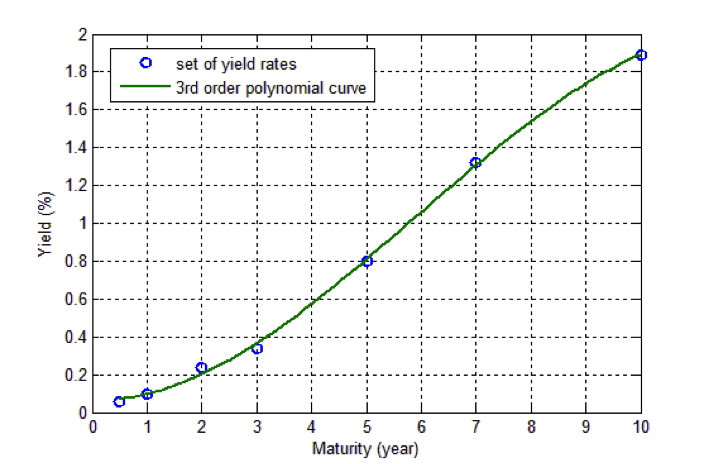
\includegraphics[width=0.75\textwidth]{prm.png}
    \end{center}
    \caption{Polynomial Regression of Yield Rate}
\end{figure}


\subsection{Asset Selection}
\vspace{8pt}
In this section, we will choose around 30 assets to construct a portfolio to fulfill our future liability obligations. The assets are a pool of Treasury notes with different maturities. And the final selection is based on the criteria stated as follows.\\

\noindent $\bullet$ Credit Risk\\
\\
\noindent The assets we selected are all governmental bonds. This ensures that all obligations will be fulfilled without concerned of default risks. Compared to other bonds issued by corporations or municipal governments, Treasury bonds can best fulfill this criterion.\\
\\
$\bullet$ Interest Rate Risk\\
\\
Another concern for choosing the assets is interest rate risk. Since we need to know portfolio future cash flow when we construct the portfolio, we need to choose bonds with fixed payments. In this way, we eliminate TIPS, which has adjustable principals. \\
\\
$\bullet$Payment Matching\\
\\
The maturities for selected assets should match those of our liability. As presented, the payment is made semi-annually, so our assets should pay at around those dates. This is one reason we choose T-notes, which have regular semi-annual payments. To solve the problem that there is no matching bond on the exact days, we choose T-notes with maturity before the exact payment dates. Note that this is of great importance since if we choose ones after the dates, the notes will fail to meet the obligation.\\
\\
Eventually, we find 32 assets satisfying the above criteria. The portfolio is made up of non-callable T-notes and T-bonds, mostly with coupons. \footnote{The data is gathered on Yahoo!~Finance.} The portfolio assets are shown in Figure 4.2.\\
\\
\begin{figure}[htb]
    \begin{center}
        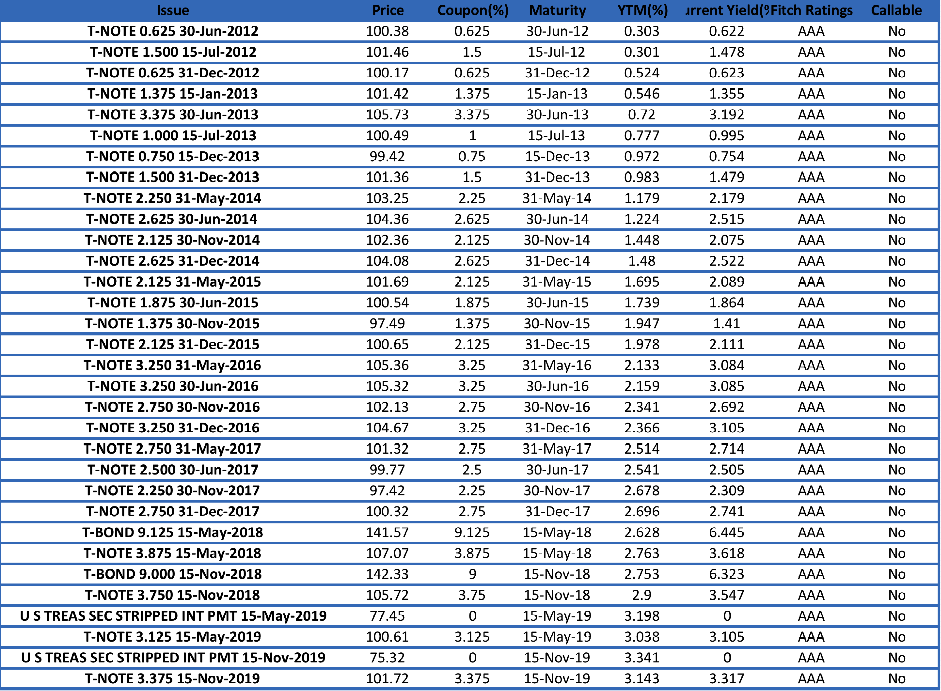
\includegraphics[width=0.75\textwidth]{finance.png}
    \end{center}
    \caption{Portfolio Assets}
\end{figure}
\subsection{Cash Flow Matching}

In this section, we are asked to construct a dedicated portfolio that can generate future cash flow to satisfy our future financial obligation.\\
\\
 We set the linear programming system in a way that by changing the weight of each bonds in our portfolio and by changing the excess cash from each period, our initial investment and the excess cash from each period will be minimized. \\
\\
In order to achieve so, we imposed two constraints. \\
\\
\noindent $\bullet$ All expected cash flow from the bond portfolio must exceed the expected liability in the same period.\\
\\
$\bullet$ All the weights of the bonds in the portfolio must be positive.  \\
\\
Then the rest of work is to solve the linear programming and conduct related analysis on our outcomes. These will be explained in details in the following chapters.

\subsection{Immunization}
\vspace{8pt}
The linear program is set up as follows:\\

\noindent $\bullet$ Minimize total price of the bond portfolio\\
\noindent $\bullet$ Change non-negative quantity (or weight) of each bond\\
\noindent $\bullet$ Subject to: duration, convexity and present value of the bond portfolio are equal to those of the liability stream.\\

\begin{table}[h]
\centering  
\begin{tabular}{cccc}
\hline
Feature  &Amount\\ \hline  
Total Price  &113.2814 million dollars\\
Total Duration  &7.85432\\ 
Total Convexity  &86.74968\\ 
Total PV  &119.8625 million dollars\\ 
\hline
\end{tabular}
\caption{Bond Portfolio	}
\end{table}
 
	
	


\chapter{Results}\label{}

By solving the linear programming, we get the initial cost to be 112.21 million dollars.\\

\noindent Digging into the sensitivity analysis, we graphed the zero-coupon rate implied from the shadow price and the zero-coupon rate implied from boot-trap method. Since the shadow price in period N represents the cost to buy 1 dollar in period N, the term structure of the implied interest rate should equal to the actual term structure given the assumption that all the bonds in our portfolio are risk free. From the graph, we see the two term-structures are fairly close in the period below 6-years and the jump of the graph beyond the 6th year could be attributed to the limited selection of bonds over long term.\\

\begin{figure}[htb]
  \begin{center}
      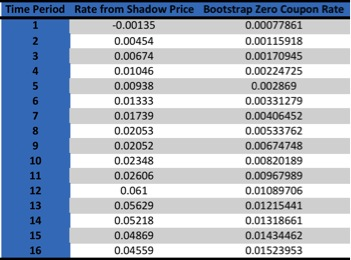
\includegraphics[width=0.75\textwidth]
{cf.jpg}
    \end{center}
    \caption{Cash Flow Matching Portfolio}
\end{figure}

\chapter{Conclusions}\label{}
		        
Our optimized portfolio, priced at 113.28 million dollars in the same units as the liability stream, is composed of 0.126 Treasury note expiring June 30, 2012, coupon rate 62.5 bp; 0.488 Treasury note expiring November 30, 2015, coupon rate 137.5 bp; and 0.373 Treasury bond expiring November 15, 2018, coupon rate 375 bp. Because we only have three non-trivial constraints, three instruments suffice, whereas in cash flow matching we have an overloaded program requiring a dozen kinds of bonds for the solution.\\

\noindent Note that the price, 113.28 million dollars, is slightly higher than what we have reported in cash flow matching. We tried having the excess cash in each period non-negative, only to find that this one more constraint render the linear program infeasible. If we relax this constraint a little, say, maximally 5 in the red every month, we will still reach a solution very close to what we already have. In this sense, we may conclude that our solution is robust, and the fundamental challenge lies in the screening of the bonds.

%\include{D_Analysis}
%\include{E_Results}
%\include{F_Conclusion}

%\include{chapter1}
%\include{chapter2}
%\include{chapter3}
%\include{chapter4}
%\include{chapter5}
%\include{chapter6}


\appendix
\ifthenelse{\boolean{@twoside}}{\myclearpage}{}
\chapter{Programming Code}\label{Programming Code}
\section{Yield Rates Calculation}
We obtained daily treasury yield curve rates from the website of U.S. Department of Treasury. \footnote{Data Source: \\
http://www.treasury.gov/resource-center/data-chart-center/interest-rates/Pages/TextView.aspx?data=yield} 
\begin{lstlisting}
maturity = [0.5 1 2 3 5 7 10]; % (years)
yield = [0.06 0.10 0.24 0.34 0.80 1.32 1.89]; % 01/13/12 (percent)
 
order = 3; % 3rd order polynomial curve fitting
p = polyfit(maturity, yield, order);
 
n = 100; % # of samples to draw a fitted curve
x = linspace(min(maturity(:)), max(maturity(:)), n); % time in year
y = polyval(p,x); % fitted curve
plot(maturity, yield, 'o', x, y, 'LineWidth', 2); xlabel('Maturity (year)')
ylabel('Yield'), legend('set of yield rates', '3rd order polynomial curve')
grid on
 
startDate = '1/15/2012';
endDate = ['7/15/2012'; ... '1/15/2020']; % given data
 
liability = [6 6 9 9 10 10 10 10 8 8 8 8 6 6 5 5]'; % given data (M$)
 
yearFraction = yearfrac(startDate, endDate); % (year)
rate = polyval(p, yearFraction); % (percent)
factor = (1+rate/100).^-yearFraction; % (1+r)^-t
PV = liability .* factor; % (M$)
sumPV = sum(PV) % (M$)
 
table = [liability yearFraction rate factor PV];


\end{lstlisting}
\chapter{Glossary}\label{Glossary}

\vspace{12pt} 

\vspace{8pt}
\noindent {\bf Cash Flow Matching}. The strategy used to construct a portfolio that will fund a schedule of liabilities from a portfolio's cash flows, with the portfolio's value diminishing to zero after payment of the last liability. 

\vspace{8pt}
\noindent {\bf Immunization}. A hybrid strategy having elements of both active and passive strategies . It's used to minimize reinvestment risk over a specified investment horizon.\\
There are three necessary conditions to assure multiple liability immunization:
1) Present value of the assets must equal the present value of the liabilities
2) The composite portfolio duration must equal the composite liabilities duration
3) The distribution of durations of individual assets in the portfolio must have a wider range than the distribution of the liabilities


\vspace{8pt}
\noindent {\bf Bootstrapping}. In finance, bootstrapping is a method for constructing a (zero-coupon) fixed-income yield curve from the prices of a set of coupon-bearing products, e.g. bonds and swaps.

\vspace{8pt} \noindent {\bf Duration}. In finance, the duration of a financial asset that consists of fixed cash flows, for example a bond, is the weighted average of the times until those fixed cash flows are received. When an asset is considered as a function of yield, duration also measures the price sensitivity to yield, the rate of change of price with respect to yield or the percentage change in price for a parallel shift in yields.



\ifthenelse{\boolean{@twoside}}{\myclearpage}{}

%\endinput

% Add your bibliography to Contents
\ifthenelse{\boolean{@twoside}}{\myclearpage}{\newpage}
\addtocontents {toc}{\protect \contentsline {chapter}{REFERENCES}{}}
\addcontentsline{toc}{chapter}{Selected Bibliography Including Cited Works}  

\newpage
\begin{thebibliography}{4}  
\bibitem{} Menchero, Jose and Benjamin Davis, 2007, ``Risk Contribution is Exposure Times Volatility Times Correlation," \emph{The Journal of Portfolio Management, 37(1).} 
\bibitem{}  Winkelmann, Kurt, Scott McDermott, Alain Kerneis and Yevgenia Zemlyakova, 2007, ``Liability-Driven Investment Policy: Structuring the Hedging Portfolio," \emph{Goldman Sachs Asset Management Strategic Research.}
\bibitem{}  Ross, S., 1976, ``Options and Efficiency," \emph{Quarterly Journal of Economics, 90.}
\bibitem{}  Bates, D., 2001, ``The Market for Crash Risk," \emph{University of Iowa.}
\end{thebibliography}


% Bibliography must come last.
\bibliographystyle{plain}
\renewcommand\bibname{Selected Bibliography Including Cited Works}
\nocite{*}  % List ALL references in your references, not just the ones cited in the text.
% This scheme automatically alphabetizes the Bibliography.
\bibliography{Biblio}
\end{document}
